% Created 2016-09-01 Qui 14:33
\documentclass[12pt,xcolor=dvipsnames,presentation,handout]{beamer}
\usepackage[utf8]{inputenc}
\usepackage[T1]{fontenc}
\usepackage{fixltx2e}
\usepackage{graphicx}
\usepackage{grffile}
\usepackage{longtable}
\usepackage{wrapfig}
\usepackage{rotating}
\usepackage[normalem]{ulem}
\usepackage{amsmath}
\usepackage{textcomp}
\usepackage{amssymb}
\usepackage{capt-of}
\usepackage{hyperref}
\graphicspath{{../}}
\usedescriptionitemofwidthas{bl}
\usepackage[T1]{fontenc}
\usepackage[utf8]{inputenc}
\usepackage{ifthen,graphicx,amsmath,amstext,gensymb,amssymb}
\usepackage{boxedminipage,xspace,multicol}
\usetheme{Madrid}
\usecolortheme[named=NavyBlue]{structure}
\useinnertheme{circles}
\setbeamertemplate{footline}[frame number]
\setbeamertemplate{navigation symbols}{}
\usepackage{verbments}
\usepackage{xcolor}
\usepackage{color}
\usepackage{url} \urlstyle{sf}
\usepackage[american]{babel}
\usepackage{pdfpages}
\usepackage{relsize}
\usepackage{tikzsymbols}
%\usepackage{tabularx}
%\usepackage{booktabs}
\def\smiley{\Smiley[1][green!80!white]}
\def\frowny{\Sadey[1][red!80!white]}
\def\winkey{\Winkey[1][yellow]}


% #+LATEX_HEADER: \usedescriptionitemofwidthas{bl}
% #+LATEX_HEADER: \usepackage[T1]{fontenc}
% #+LATEX_HEADER: \usepackage[utf8]{inputenc}
% #+LATEX_HEADER: \usepackage[american]{babel}
% #+LATEX_HEADER: \usepackage{ifthen,figlatex,amsmath,amstext,gensymb,amssymb}
% #+LATEX_HEADER: \usepackage{boxedminipage,xspace,multicol}
% #+LATEX_HEADER: %%%%%%%%% Begin of Beamer Layout %%%%%%%%%%%%%
% #+LATEX_HEADER: \ProcessOptionsBeamer
% #+LATEX_HEADER: \usecolortheme{whale}
% #+LATEX_HEADER: \usecolortheme[named=BrickRed]{structure}
% #+LATEX_HEADER: \useinnertheme{rounded}
% #+LATEX_HEADER: \useoutertheme{infolines}
% #+LATEX_HEADER: \setbeamertemplate{footline}[frame number]
% #+LATEX_HEADER: \setbeamertemplate{headline}[default]
% #+LATEX_HEADER: \setbeamertemplate{navigation symbols}{}
% #+LATEX_HEADER: \defbeamertemplate*{headline}{info theme}{}
% #+LATEX_HEADER: \defbeamertemplate*{footline}{info theme}{\leavevmode%
% #+LATEX_HEADER:   \hbox{%
% #+LATEX_HEADER:     \begin{beamercolorbox}[wd=.2\paperwidth,ht=2.25ex,dp=1ex,center]{author in head/foot}%
% #+LATEX_HEADER:       \usebeamerfont{author in head/foot}\insertshortauthor
% #+LATEX_HEADER:     \end{beamercolorbox}%
% #+LATEX_HEADER:   \begin{beamercolorbox}[wd=.71\paperwidth,ht=2.25ex,dp=1ex,center]{title in head/foot}%
% #+LATEX_HEADER:     \usebeamerfont{title in head/foot}\insertsectionhead
% #+LATEX_HEADER:   \end{beamercolorbox}%
% #+LATEX_HEADER:   \begin{beamercolorbox}[wd=.09\paperwidth,ht=2.25ex,dp=1ex,right]{section in head/foot}%
% #+LATEX_HEADER:     \usebeamerfont{section in head/foot}\insertframenumber{}~/~\inserttotalframenumber\hspace*{2ex} 
% #+LATEX_HEADER:   \end{beamercolorbox}
% #+LATEX_HEADER:   }\vskip0pt}
% #+LATEX_HEADER: \setbeamertemplate{footline}[info theme]
% #+LATEX_HEADER: %%%%%%%%% End of Beamer Layout %%%%%%%%%%%%%
% #+LATEX_HEADER: \usepackage{verbments}
% #+LATEX_HEADER: \usepackage{xcolor}
% #+LATEX_HEADER: \usepackage{color}
% #+LATEX_HEADER: \usepackage{url} \urlstyle{sf}


\institute{
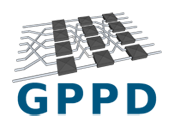
\includegraphics[width=.16\textwidth]{img/gppd.png}
\hfill

\includegraphics[width=.16\textwidth]{img/inf.pdf}
\hfill

\includegraphics[width=.16\textwidth]{img/ufrgs.pdf}
% \hfill
% 
\includegraphics[width=.16\textwidth]{img/cnpq.pdf}
\hfill

\includegraphics[width=.18\textwidth]{img/hpe.png}
}
\usetheme{default}
\author{Gabriel B. Moro and Lucas M. Schnorr \\ \{gbmoro,schnorr\}@inf.ufrgs.br}
\date{XIV Workshop de Processamento Paralelo e Distribuído \linebreak UFRGS, Porto Alegre, 2nd September 2016}
\title{Measuring Hardware Counters for HPC Application Phase Detection}
\hypersetup{
 pdfauthor={Gabriel B. Moro and Lucas M. Schnorr \\ \{gbmoro,schnorr\}@inf.ufrgs.br},
 pdftitle={Measuring Hardware Counters for HPC Application Phase Detection},
 pdfkeywords={},
 pdfsubject={},
 pdfcreator={Emacs 24.3.1 (Org mode 8.3.5)}, 
 pdflang={English}}
\begin{document}

\maketitle

\let\alert=\structure % to make sure the org * * works
\def\n{\\\hline}             
\def\eg{e.g.,\xspace}
\def\Eg{E.g.,\xspace}
\def\ie{i.e.,\xspace}
\let\alert=\structure
\let\epsilon=\varepsilon
%\let\leq=\leqslant
%\let\geq=\geqslant
\def\R{\ensuremath{\mathbb{R}}\xspace}
\def\F{\ensuremath{\mathcal{F}}\xspace}
\def\N{\ensuremath{\mathcal{N}}\xspace}
\def\P{\ensuremath{\operatorname{P}}\xspace}
\def\E{\ensuremath{\operatorname{E}}\xspace}
\def\Var{\ensuremath{\operatorname{Var}}\xspace}
\def\rv#1{\ensuremath{\textcolor{blue}{#1}}\xspace} % DarkBlue

\def\RR{\ensuremath{R^2}\xspace}


\makeatletter
\gdef\fsvtpage{\ps@navigation\refstepcounter{framenumber}}%
\makeatother
\setbeamercolor{background canvas}{bg=}

\definecolor{keywords}{RGB}{255,0,90}
\definecolor{comments}{RGB}{60,179,113}
\definecolor{fore}{RGB}{249,242,215}
\definecolor{back}{RGB}{51,51,51}
\newcommand{\accolade}[1]{$\left\{\begin{array}{c}\vspace{#1}\end{array}\right.$}
%\lstset{
%  basicstyle=\color{fore},
%  keywordstyle=\color{keywords},
%  commentstyle=\color{comments},
%  backgroundcolor=\color{back}
%}

\newcommand{\restorefootline}{\setbeamertemplate{navigation symbols}{}}
\newcommand{\setfootline}[1]{\setbeamertemplate{navigation symbols}{\textcolor{black}{\textbf{#1}}}}
\newcommand{\includeslides}[3]{%
  \setfootline{#1}%
  \includepdf[pages={#2},pagecommand={\fsvtpage},turn=false,noautoscale=false,column=false,columnstrict=false,openright=false]{pdf_sources/#3}%
%  \includepdf[pages={#2},pagecommand={\fsvtpage},scale=.8,offset=20
%  -23,turn=false,noautoscale=false,column=false,columnstrict=false,openright=false]{pdf_sources/#3}%
  \restorefootline%
}
\end

\def\recurrenttoc{%
\makeatletter
\AtBeginSection[]
{
  \frame<handout:0>
  {
    \frametitle{Outline}
    \tableofcontents[current,currentsubsection]
  }
}
\makeatother
}

\newcommand{\bottomcite}[1]{\fbox{\vbox{\footnotesize #1}}}

\newcommand{\prettysmall}[1]{\fontsize{#1}{#1}\selectfont}

\section{Introduction}
\label{sec:orgheadline3}
\subsection{}
\label{sec:orgheadline2}
\begin{frame}[fragile,label={sec:orgheadline1}]{Introduction}
 \texttt{Motivation}:

\begin{itemize}
\item Reducing the power consumption of parallel applications;
\item Fine-granularity to identify the \uline{memory-bound regions} of parallel
application several timestamps;
\item \uline{Lower overhead} of measurement.
\end{itemize}

\texttt{Objective}:

\begin{itemize}
\item Measure hardware counters at every given time interval to discover
memory-bound regions
\end{itemize}
\end{frame}

\section{Related Works}
\label{sec:orgheadline7}
\subsection{}
\label{sec:orgheadline6}
\begin{frame}[fragile,label={sec:orgheadline4}]{Related Works}
 \texttt{Spiliopoulos et al}:
\begin{itemize}
\item Tool that analyzes the behavior of sequential application (the
concept of phases);
\item Based on cache misses of different caches' levels.
\end{itemize}

\texttt{Laurenzano et al}: 
\begin{itemize}
\item Finer granularity for each application loop.
\end{itemize}

\texttt{Freeh et al.}:
\begin{itemize}
\item Define the most suitable frequency for each phase of MPI
applications;
\item Analyse of the best frequency for each node.
\end{itemize}
\end{frame}


\begin{frame}[label={sec:orgheadline5}]{References}
\tiny
\bibliographystyle{plain}
\bibliography{europar2016}
\end{frame}
\end{document}
